% 22 pages
This chapter will lay foundations for medical imaging for clinical diagnostics and the basic methodology used throughout this thesis to tackle advanced imaging diagnostics.

\section{Clinical Background: Volumetric Medical Imaging} %7 pages

% Ideas:
% zhang2024challenges (foundation models in deep learning)
% https://3dqlab.stanford.edu/what-is-3d-imaging-2/

    \subsection{Diagnostic Disciplines and Tasks} % 2 pages
        With the development of the CT scanner by Godfrey Hounsfield in the late 1960s, taking volumetric images of the body became possible and was used and researched with increasing effort in the following decades \citep{alexander2010emi, rubin2014computed}. Volumetric \ac{CT} images can be used to diagnose and plan the treatment of several diseases and conditions such as stroke, vascular diseases, cancer (see \chapref{chap:deepstaple}), trauma, acute abdominal pain and diffuse lung disease \citep{rubin2014computed}. With volumetric \ac{CT} images an exact evaluation of  three-dimensional measures such as tumor growth and estimation
        of doubling times % (271) TODO orig source of doubling times
        and analyzing the three-dimensional shape became possible \citep{rubin2014computed}. Similarly other volumetric quantities could be measured such as the volume of the
        left cardiac ventricle,  % TODO orig source (343)
        cerebral spinal fluid, % TODO orig source (344)
        liver and spleen % TODO orig source (345)
        and tumoral neoplasia. % TODO orig source (346)
        CT in its current state has excellent spatial resolution and distinguishing tumors given that tumors and the surrounding tissue provide enough contrast \citep{abramson2023surgeons}.
        But the three primary objectives of radiologists, namely the detection, resolution and characterization of abnormalities \citep{abramson2023surgeons} might not be satisfied when tissue does not provide enough contrast on X-ray beams.
        % utting-edge CTtechniques, including the use of more sensitive photon counting de-tectors3 and dual energy data acquisition,4,5 will increase CT spatial resolution and contrast while minimizing noise, but this is unlikely toovercome the multitude of MR sequences tailored to images varioustissues throughout the body.  \citep{abramson2023surgeons}

        \ac{MRI}, which is available commercially since the early 1980s, has superior contrast over CT regarding soft-tissue \citep{abramson2023surgeons, kabasawa2022mr}. \ac{MRI} sequences can be specifically tailored towards the application regarding. This requires a trade-off beetween sufficient \ac{SNR}, voxel volume and acquisition time under the influence of the examined object\footnote{A more in-depth explanation can be found in \ref{chap:acquisitionfocus}} \citep{macovski1996noise}. E.g. T2 sequences suppressing fat are excellent for tumor detection, where tumors are displayed brighter than the dark, suppressed fat, but spatial resolution is rather coarse with 5mm thick slicing gaps \citep{abramson2023surgeons}.
        \ac{MRI} can be used in various applications such to assess brain and heart function (see \chapref{chap:deepstaple} and \chapref{chap:acquisitionfocus}), abdominal organs such as liver and pancreas (see \chapref{chap:dgtta}) and knee cartilage \citep{mazurowski2019deep}.

        TODO insert segmentation, registration, shape reconstruction, data hires / data reconstruction

        % Within this con-text, the need to reformat, reconstruct,and render CT images into alternativedisplays was driven by a desire to pro-vide all physicians with an understand-ing of the anatomic nuances that CT provided in a manner that might been countered in the surgical suite. Al-though computers and computation arefundamental to CT, the applications ofcomputer graphics, vision, and quan-titation methods were not sufficientlymature to make their use routine un-til the latter days of the 20th century. \citep{rubin2014computed}


        % s. One quickly meet challenges associated to memoryand compute consumption when using CNNs with higher-dimensional image data, challenges thatresearchers are trying various approaches to deal with (treating 3D as stacks of 2Ds, patch- orsegment-based training and inference, downscaling, etc). It is clear that the ideas behind state-of-the-art two-dimensional CNNs can be lifted to three dimensions, but also that adding a thirdspatial dimension results in additional constraints. \citep{lundervold2019overview}

        % DL specific
        % \citep{litjens2017survey}
        % \citep{piccialli2021survey}

        % TODO Why is US not explained in this thesis?

        % How did volumetrict Medical Imaging evolve
        % CT and MRI are often done paired follow ups? This is why these are in focus.
        % CT (and PET) and MRI are important imaging domains.

    \subsection{Imaging Domains and Scanner Properties} % 2.5 pages
        \label{sec:imaging_domains}
        \begin{figure}
            \begin{minipage}{\textwidth}
                \centering
                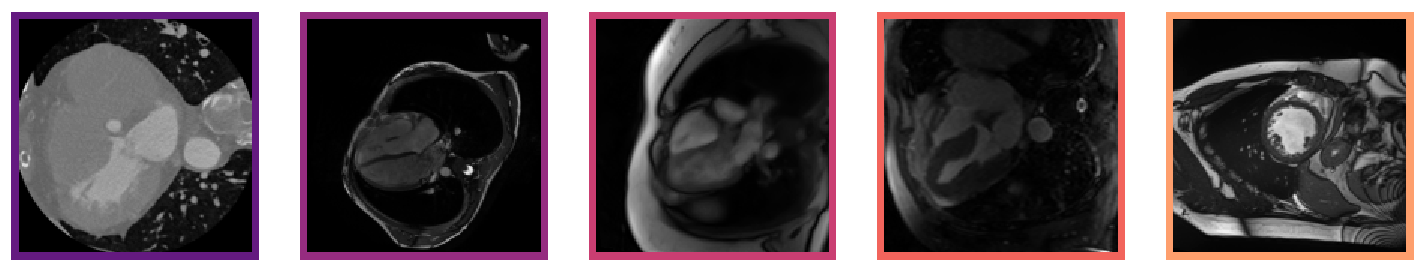
\includegraphics[width=.89\textwidth]{sections/02_background/figures/contrast_imgs.pdf}
                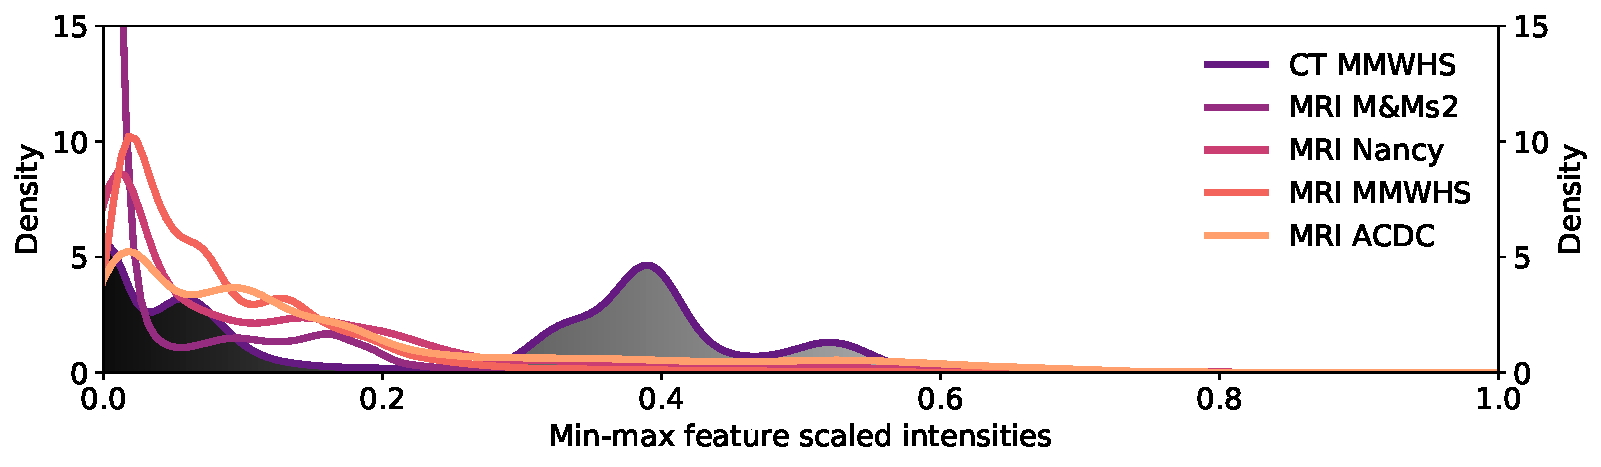
\includegraphics[width=\textwidth]{sections/02_background/figures/contrast_histograms.pdf}
                \caption{Top: One \ac{CT} and several \ac{MRI} images of cardiac studies and one internal dataset (Nancy) \citep{zhuang2019evaluation,martin2023deep,
                campello2021multi,bernard2018deep}. Bottom: Histogram of the image intensities each scaled to min-max feature scales. The \ac{CT} histogram is shaded with the corresponding image grayscale intensities. Appearance of \ac{CT} and \ac{MRI} images differ substantially but also \ac{MRI} images have a large variation in appearance due to different scanners and acquisition protocols. Similar findings are presented in \citep{guan2021domain}.}
                \label{fig:domain_contrast}
            \end{minipage}
        \end{figure}

        Due to the different acquisition principles of \ac{CT} and \ac{MRI} scanners and the adjustability of \ac{MRI} scanner sequences the appearance of images showing the same content can differ substantially as shown in \figref{fig:domain_contrast} forming multiple imaging \emph{domains} and as per definition an imaging domain contains data of the same distribution \citep{wang2022generalizing}.

        In a \ac{CT} scanner, X-ray beams are emitted and detected after the beams have been influenced by the matter and tissue of interest according to Beer-Lamberts law given in \eqqref{eq:beer_lambert}, where $I_0$ initially transmitted X-ray intensity and $I$ the output intensity influenced by $n$ materials with linear attenuation coefficient $\mu_i$ and path length $x_i$ through each material. Differences in attenuation coefficients between materials and different sizing contributes to a larger \emph{attenuation contrast}. For soft tissue which does not yield sufficent attenuation contrast, \emph{phase contrast} can be utilized to improve distinction.
        The materials' refractive index $n_r$ consists of factor $\beta$ influencing the aforementioned attenuation process and $\delta$ responsible for phase changes of the X-ray waves that pass the object described by \eqqref{eq:refractive_index} \citep{withers2021x}.

        \begin{minipage}[b]{.45\textwidth}
            \begin{align}
                I &= I_0 e^{-\sum_{i=1}^{n} \mu_i x_i} \label{eq:beer_lambert} \\
                n_r &= 1-\delta + i\beta \label{eq:refractive_index}
            \end{align}
        \end{minipage}
        \hfill
        \begin{minipage}[b]{.45\textwidth}
            \begin{align}
                M(\tau) &= M_0(1-e^{-\nicefrac{\tau}{T_1}}) \label{eq:T1decay}\\
                M_{xy}(\tau) &= M_{xy,max}(e^{-\nicefrac{\tau}{T_2^*}})\label{eq:T2decay}
            \end{align}
        \end{minipage}
        \vspace{6pt}

        \begin{minipage}[b]{.45\textwidth}
            \ac{CT}: Basic equations describing the physical principle of \ac{CT} imaging \citep{withers2021x}.
        \end{minipage}
        \hfill
        \begin{minipage}[b]{.45\textwidth}
            \ac{MRI}: Basic equations describing the measurable magnetic field intensity decay in \ac{MRI} \citep{dale2015mri}.
        \end{minipage}
        \vspace{12pt}

        Medical \ac{CT} scanners typically use rotating gantry systems containing several sources and detectors or stationary cone-beam systems \citep{withers2021x}. The spatial resolution of the scan is contrained by geometrical properties --- the detectors' sizes, their number, their distances to the X-ray sources and on the size of the X-ray focal spot \citep{withers2021x}.

        \ac{MRI} images are generated by a completely different physical principle. Hydrogen nuclei in water or fat, whose single proton has a nuclear spin that creates a tiny magnetic field. In an external magnetic field $B_0$ these protons align to the field either towards or against the field direction \citep{ridgway2010cardiovascular} ($z$-direction as per definition). On a macroscopic scale, all hydrogen nuclei within the tissue form a measurable net magnetization $M_0$ after a short time of alignment. The nuclei can now be influenced by an \ac{RF}-pulse with a magnetic field rotation at Larmor frequency $\omega_0 = \gamma B_0$, disturbing the equilibrium and turning them towards the $xy$-plane of the scanner. This happens in a rotational motion called precession also at the Larmor frequency $\omega_0$, where $\gamma$ is the gyromagnetic ratio which is constant. After turning off the \ac{RF}-pulse a changes of magnetic fields $M$ and $M_{xy}$ can be measured externally. The change of magnetic fields happens at certain decay rates $T_1$ and $T_2^*$, specific to the tissue that is examined \eqqref{eq:T1decay} and \eqref{eq:T2decay} \citep{withers2021x}. Exponential $T_1$-decay (also called relaxation) measures the return of nuclei to the initial magnetization $M_0$ and $T_2^*$-decay measures the decay of net magnetization in the $xy$-plane regarding that the nuclei with precession motion loose their phase, which results in a stronger decay over time.
        The MRI device needs to contain several electrical coils to generate and measure the magnetic fields (main magnetic coils, \ac{RF}-pulse coils). To retrieve information of the tissue in three dimensions, additional gradient coils are needed to alter the effective main field strength spatially \citep{ridgway2010cardiovascular}. Given, that \ac{RF}-pulses are only effective for a certain Larmor frequency that is dependent on the effective main field strength, it is possible to only excite hydrogen nuclei inside a specific spatial region \citep{ridgway2010cardiovascular}. This enables a dynamic selection of imaging slices, and to track magnetic signals down to specific positions inside that slice which can be used to compose the k-space data and the final image after applying a \ac{2D}-Fourier transform \citep{ridgway2010cardiovascular}.
        Given that principle, different types of \ac{RF}-pulses can be applied, forming a vast possibility of imaging sequences that e.g. either emphasize tissue with prominent $T_1$ or $T_2^*$ values --- generating $T_1$- or $T_2^*$-weighted images or a mixture. This makes \ac{MRI} a versatile tool for soft-tissue examination.
        % What are the special benefits and downsides of CT, MRI, technically speaking.

        % example images
        % Value ranges (histogram) https://pmc.ncbi.nlm.nih.gov/articles/PMC9011180/pdf/nihms-1794910.pdf
        % Image normalization by scanner (HU vs. MRI)
        % MRI magic triangle T1 weighted / T2 weighted scans
        % slicing MRI vs CT
        % image recovery: MRI k-Space transform, CT Radon transform
        % Acquisition timing
        % Scanner costs

    \subsection{Generalization: Challenges and Possibilities} % 2.5 pages
        In case of deep learning, where an algorithm is used to train a model on existing data from a \emph{source} domain (see \secref{sec:deep_learning}), the usage of this trained model on another \emph{target} domain often leads to performance degradation, as presented in this section.
        This can be shown even for low-dimensional data tasks, where optimal and less optimal ratios of source and target data used in the training phase of the model can theoretically be derived \citep{ben2010theory}.
        In \ac{2D}-tasks, such as the classification of several thousand images of the ImageNet dataset, this performance decline was even shown after the commonly used training and test data selection (refered to as data split) was altered for models that were optimized solely under the unaltered data split \citep{recht2019imagenet}. This example shows, that defining different domains is a non-trivial task and boundaries can be blurred.
        % \citep{recht2019imagenet}  ence the third term is the standard generalization gap commonly studied in machinelearning. It is determined solely by the random sampling error.
        % \citep{recht2019imagenet}  cenario. So at least on CIFAR-10 and ImageNet, multiple yearsof competitive test set adaptivity did not lead to diminishing accuracy numbers.
        % The lack of diminishing returns in our experiments points towards the distribution gap as the primaryreason for the accuracy drops. Moreover, our results on ImageNet show that changes in the samplingstrategy can indeed affect model accuracies by a large amount, even if the data source and otherparts of the dataset creation process stay the same. \citep{recht2019imagenet}

        \paragraph{Challenges} Given that trained deep learning models suffer performance degradation under shifts of the data domain, several challenges arise for volumetric medical imaging tasks comprising images of scanners with different acquisition principles and sequence properties (see \secref{sec:imaging_domains}).
        First of all, the lack of data and labeled data restricts the training of deep learning models to be conducted in a limited number of source domains (and often only one domain) \citep{guan2021domain}.
        This becomes more severe if deep learning models for less prominent imaging techniques such as \ac{MRI} with radial instead of orthogonal sampling patterns are studied \citep{han2018deep}.
        Leveraging models pretrained on a large amount of natural image data (e.g. from the mentioned ImageNet dataset) may be helpful, but using \ac{2D} models for \ac{3D} images does not access all information shared between image layers in the volumetric image \citep{guan2021domain}.
        Even if in general the same imaging sequence is used such as \ac{SSFP}, image domain shifts can be severe enough between multiple vendors to diminish the results of deep learning models as shown in a segmentation task for GE, Siemens and Philips scanners \citep{yan2019edge}.
        Image content changes can even be undistinguishably small so that changes cannot be observed by humans but results for deep learning based algorithms may vary by a large margin. This was shown also shown for medical image tasks with adversarial perturbations made to the input images in cardiac segmentation \citep{yan2019domain}.
        Explicitly leveraging the knowledge of different domains can lead to improve generalization abilities \citep{ganin2016domain}. But this requires to forcably label image sets with a domain label --- which is difficult regarding that even slightest changes can form a new domain.

        \paragraph{Possibilities} The mentioned challenges on the other hand give rise to solutions for generalizing approaches.
        % 12/10 methods giving answers MRI CT
        The problem of data scarcity in \ac{MRI} with specific, rare sequences i.e. can be solved by leveraging larger-scales \ac{CT} as seen in \citep{han2018deep}.
        Extracting edge-features of the image may serve as a robust intermediate training step to cope with multi-vendor \ac{MRI} data\citep{huang2022online}.
        Scores in cross-site segmentation can effectively be recovered with pretraining on large-scale computer-vision datasets when the correct input prompting mechanisms are delivered for medical imaging data \citep{gao2024desam}.
        Moreover, specifically designed shape constraints for the target organs can improve model generalization for T2-weighted cross-site \ac{MRI} data \citep{liu2020shape}.
        Cross-modality segmentation between \ac{MRI} and \ac{US} can be improved with intensive data augmentation \citep{zhang2020generalizing} for different tasks such as heart or prostate segmentation. Overcoming a domain gap from \ac{MRI} and \ac{CT} domains is likewise improved with targeted augmentation schemes \citep{ouyang2022causality}.

        Depending on the target task at hand, the generalization approaches can be specifically tailored (apart from medical image segmentation that is extensively studied for volumetric images).
        Alzheimer classification was improved using structural-causal-models in \citep{wang2021harmonization} in brain \ac{MRI}. Landmark detection on medical data was enabled for different unlabeled domains leveraging domain-specific and domain-shared model parts  \citep{zhu2023uod}. Registration of \ac{CT} and \ac{MRI} volumes becomes possible by extracting robust, hand-crafted image features and a coupled optimization approach \citep{siebert2021fast}. And also image reconstruction for multiple domains of \ac{CT} image kernels is feasible by using generator-guided constrastive learning approaches \citep{choi2023ct}. Joint intra-domain image features of \ac{PET} and \ac{MRI} can be combined to improve the reconstruction of undersampled \ac{MRI} data \citep{gautier2024bimodal}.


        % and emphysema classification by using
        %  alzheimer disease Classification
        % \citep{cheplygina2019not} emphysema classification in CT: Learning scenarios, illustrated by a task of classifying healthy (green) vs emphysema (red) tissue in chest CT images (only a meta paper)


        % TODO integrate these basics about DG / DA etc
        % As described in xx generalizatoin needs xyz

        % % \citep{yan2019domain} shift: transfer learning > domain adaptation
        % % data: domain generalization > domain adaptation % TODO integrate this into a generalization / domain adaptation paragraph

        % OVERVIEW OF BENCHMARK DATASETS FOR DOMAIN ADAPTATION RESEARCH ON DIFFERENT MEDICAL IMAGE ANALYSIS TASKS. \citep{guan2021domain}

        % \citep{guan2021domain} survey on domain adaptation


        % \citep{wang2022generalizing} in recent years, Domaingeneralization (DG) has received much attention. As shownin Fig. 1, the goal of domain generalization is to learn amodel from one or several different but related domains (i.e.,diverse training datasets) that will generalize well on unseentesting domains.

        % The goal of domain generalization is to learn a robust andgeneralizable predictive function h : X  Y from the M training domains to achieve a minimum prediction error on an unseentest domain Stest:

        % A domain is composed of data that aresampled from a distribution.

        % The joint distributions between each pairof domains are different: P

        % The goal of domain generalization is to learn a robust andgeneralizable predictive function h : X → Y from the M training
        % domains to achieve a minimum prediction error on an unseentest domain Stest (i.e.,

        % \citep{yang2024generalized}




\section{Methodological Background: Deep Learning} % 15 pages
    \label{sec:deep_learning}
    % TODO: This needs to be a lot shorter now
    % https://books.google.de/books?hl=de&lr=&id=qOF4AgAAQBAJ&oi=fnd&pg=PP1&ots=vNTiX5Lu_U&sig=UEC7rljJ7dVsAbh_XQeMmCrNqcU#v=onepage&q&f=false
    The principal mechanisms of learning were studied in the last century by investigating conditioned learning, where an outcome is associated to a stimulus by a learning organism e.g. a dog that awaits food after hearing the sound of a bell \citep{pavlov1928conditioned, pavlov2010conditioned, banich2011generalization}. Later, fear responses were especially studied and two sub-mechanisms of conditioned learning --- generalization and specialization --- were discovered \citep{banich2011generalization}.
    In fear learning, initially an instance-based generalization occurs that maps a novel fear to an environment \citep{banich2011generalization}. Later, this generalization is specialized and mapped to specific environmental stimuli leading to discrimination \citep{banich2011generalization}.
    It was discovered, that generalization can occur intra-modal and cross-modal for the example of the food awaiting dog either receiving visual or auditory stimuli \citep{pavlov1928conditioned} and that gradients of generalization exist \citep{guttman1956discriminability}.
    The concept of gerneralization and spezialization can be tracked down to individual parts of the brain, where the initial generalized learning is associated to the amygdala whereas the specialization occurs in the prefrontal cortex and the hippocampus \citep{banich2011generalization}.

    On the cell level, learning and building memory is assumed to work as the change of neuron connection-strength through synaptic plasticity \citep{do1949organization,martin2000synaptic}. Apart from synaptic information exchange it was also figured out that information exchange occurs volumetrically between glia cells and neurons with extracellular vesicles in the nervous system \citep{schiera2019communcation}.

    \subsection{Basic Principles} % 2 pages
        % https://cs.stanford.edu/people/eroberts/courses/soco/projects/neural-networks/History/history1.html

        Inspired by the research findings in biological learning processes, \citeauthor{mcculloch1943logical} decribed several parts of network structures mimicking neural systems \citep{mcculloch1943logical}.
        Over a decade later \citeauthor{rosenblatt1957perceptron} developed the concept of a \emph{perceptron} as a learning element for electronic or electromechanical systems to recognize patterns \citep{rosenblatt1957perceptron}.
        First real classification experiments were conducted by \citeauthor{widrow1960adaptive} using small neural networks \citep{widrow1960adaptive}.
        % TODO: were those exp based on value tables? vs. backprop?
        More than two decades later the \emph{Backpropagation} mechanism was developed, that is nowadays used in current deep learning approaches to systematically configure the weights and biases of neural networks \citep{rumelhart1986learning}.

        % With increasing computational power and availability of large data through the internet machine learning techniques experienced increased interest \citep{xx}.

        \paragraph{Backpropagation} The basic principle of deep learning is the backpropagation mechanism.

        \begin{align}
            \diffp{E}{{y_j}} &= y_j - d_j \\
            \diffp{E}{{x_j}} &= \diffp{E}{{y_j}} \cdot \diffp{{y_j}}{{x_j}}
        \end{align}

        % Now that we know how deep learning works in general, we can have a look at individual building blocks models / data concepts / supervision tasks

    \subsection{Data Representation and Model Architectures} % 4 pages

        \subsubsection{Convolutional Neural Networks}
            % cnns, unets
            % cnn Kernels
        \subsubsection{Graph Neural Networks}
            % feature aggregation
            % rota groups, equivariance,

    \subsection{Training and Optimization Strategies} % 5 pages
        % curriculum learning, dice loss
        % metrics
    \subsection{Generalization: Approaches} % 3 pages
        % What are the current approaches in deep learning?

    \subsection{Generalization: Recent Discussion} % 1 pages
        How is the idea of AGI related to our gerneralization approach? What can be problems of AGI and why do we analyse generalization in a limited scope such as medical image analysis?
        % generalization methods